\documentclass[a4paper,10pt]{report}
\usepackage{graphicx} %for embedding images
\usepackage{url} %for proper url entries

\begin{document}
\pagestyle{headings}%
\thispagestyle{empty}%
\begin{center}%
	\Large\bf{Project Report}\\%
	\vspace{0.5cm}% 
	\huge\bf{Extraction of Questions from the Internet using a Machine Learning approach}\\%
               \vspace{1cm}% 
	\small\it{Submitted in partial fulfillment of}\\%
	\small\it{the requirements for the award of the degree of}\\%
	\vspace{0.5cm}%
	\large\bf\it{Bachelor of Technology}\\%
	\small\it{in}\\%
	\large\it{Computer Science and Engineering}\\%
	\vspace{0.5cm}%
	\Large\it {by}\\%
	\vspace{0.3cm}%
	\begin{table}[h]
		\centering
		\begin{tabular}{lr}\hline \\
			Roll No & Name \\ \\ \hline
			\\
            B090924CS & Alok Saw \\ 
            B090437CS & Jerrin Shaji George \\ 
            B090904CS & Shubhangam Agrawal \\ 
            B090006CS & Stein Astor Fernandez \\ \\ \hline 
		\end{tabular}
	\end{table}
	\Large\it {Under the guidance of}\\%
	\normalfont\bf{Dr. Priya Chandran}\\%
	\begin{figure}[!ht]
		\begin{center}
			
\includegraphics[scale=0.10]{nitclogo}\\%
		\end{center}
	\end{figure}
	\large\bf{Department of Computer Science \& Engineering}\\%
	\Large\bf{National Institute of Technology, Calicut}\\%
	\small\bf{Kerala - 673601}\\%
\end{center}%

\pagestyle{plain}
\begin{center}
	\huge{Department of Computer Science \& Engineering}\\[0.5cm]
	\normalsize
	\textsc{National Institute of Technology Calicut}\\[2.0cm]
	\emph{\LARGE Certificate}\\[2.5cm]
\end{center}
This is to certify that the project work entitled ``\textbf{Extraction of Questions from the Internet using a Machine Learning approach}'', 
submitted by Alok Saw (B090924CS), Jerrin Shaji George (B090437CS), Shubhangam Agrawal (B090904CS) and Stein Astor Fernandez (B090006CS) to National~Institute~of~Technology~Calicut towards 
partial fulfillment of the requirements for the award of the degree of Bachelor~of~Technology 
in Computer~Science~and~Engineering, is a bonafide record of the work carried out by them 
under my supervision and guidance.

\vspace*{1.5cm}
\noindent

\hfill Project Guide\\
\textbf{Place :} Calicut \hfill Dr. Priya Chandran\\
\textbf{Date :}  \hfill Professor\\

\vspace*{2cm}
\hfill Head of Department\\

\vspace*{2cm}
\hfill Office Seal\\


%-----------------------------------------------------------
%                      ABSTRACT
%-----------------------------------------------------------
%
\begin{abstract} 
We propose a Support Vector Machine based approach to extract questions pertaining to a topic from the internet.
We adapt certain features from \emph{SQUINT}~\cite{squint} to identify relevance of text and propose two new features to identify questions in a text \emph{section}.

This Machine Learning component is developed as an application which takes a topic as input and produces a list of questions related to the input topic as output.
\end{abstract}

%-----------------------------------------------------------

\renewcommand{\abstractname}{Problem Statement}
\renewcommand\bibname{References}

%--------------PROBLEM STATEMENT--------------------------

\begin{abstract}
    Given input a topic $t$, search the internet for pages which may contain questions related to $t$ and output a set $R$ comprising of relevant questions extracted from these pages.
\end{abstract}

%----------------------------------------------------------

\tableofcontents
\listoffigures

%----------------------------------------------------------
%                    MAIN BODY BEGINS
%----------------------------------------------------------

\part{Introduction}

\renewcommand{\abstractname}{Introduction}

\begin{abstract}

Today, there is a huge amount of data available on the internet. While advancements in search technologies have made searching for relevant pages trivial, each page contains a lot of irrelevant data, images and advertisements. Thus, having some way to extract only the relevant sections of data from the huge set of search results would result in massive effort and time savings. \\

There is often a need for students as well as faculty to obtain a list of questions related to certain topics while studying or teaching these topics. The internet has a vast number of such questions for any such topic, however one must know what terms to search for and then manually visit each page returned in the search results and find out such questions in a tedious manner. \\

We plan to use Machine Learning techniques to identify whether a section of text is a question and relevant to a topic and thus make an application to automate this process which will take a topic as input and return a list of questions based on the topic from the internet.
\end{abstract}

%------------------------------------------

\chapter{Literature Survey}

The trivial way of approaching this problem would be to simply search for the presence of the input topic in the various \emph{sections} and output matches --- however this would not yield a good performance and would have no way to identify questions. Teevan et al.~\cite{teevan} have discussed the relevance of using search methodologies that focus more on contextual information as opposed to simple keyword matching as that may not be enough the capture the relevant text. 

Thus rather than simple keyword matching, we must be able to identify patterns in the text \emph{sections} which make it a question and also make it relevant to the input topic. Machine Learning is a good approach to solve this problem as it finds the various patterns in the text without the need for detailed statistical analysis. \\

Arthur Samuel defines Machine Learning as \begin{quote}\emph{The field of study that gives computers the ability to learn without being explicitly programmed.}\end{quote}

\noindent Machine learning, a branch of artificial intelligence, is concerned with the design and development of algorithms that take as input empirical data and yield patterns or predictions thought to be features of the underlying mechanism that generated the data.

A learner can take advantage of examples (data) to capture characteristics of interest of their unknown underlying probability distribution. Data can be seen as instances of the possible relations between observed variables.

A major focus of machine learning research is the design of algorithms that recognize complex patterns and make intelligent decisions based on input data~\cite{wikiML}. \\

\noindent Machine learning problems can be categorized broadly into 2 categories~\cite{elements} ---

\begin{description}
	\item[Supervised Learning] The goal is to predict the value of an outcome measure based on a number of input measures.
	\item[Unsupervised Learning] There is no outcome measure, and the goal is to describe the associations and patterns among a set of input measures.
\end{description}

\noindent As our problem is to predict whether each \emph{section} is a related question or not, we see that `Supervised Learning' is the correct approach to our problem.

Joachims has also concluded~\cite{joachims} that Support Vector Machines are an effective text classification tool which uses the Supervised Machine Learning model. This is due to the high dimensionality of the feature vector~\cite{squint}.

Inoue et al.~\cite{squint} propose an SVM based approach to identify the most relevant subsection in Web pages returned by a search query (\emph{SQUINT}). They have obtained very accurate results using this model. \\

\noindent A Support Vector Machine takes a set of input data and predicts, for each given input, which of two possible classes forms the output, making it a non-probabilistic binary classifier. 

It constructs a hyperplane or a set of hyperplanes in a high-- or infinite--dimensional space, which can be used for classification, regression, or other tasks. Intuitively, a good separation is achieved by the hyperplane (called the \emph{functional margin}) that has the largest distance to the nearest training data point of any class, since in general the larger the margin, the lower the generalization error of the classifier~\cite{wikiSVM}. \\

\noindent Our problem is similar to \emph{SQUINT} with the significant challenge being the identification of questions. Thus, we explore a Support Vector Machine based approach similar to \emph{SQUINT} in order to detect relevance to the input topic and aim to identify various features which indicate that a \emph{section} is a question.

%----------------------------------------------------------

\part{Work Done in S7}

\chapter{Architecture}

We identified a component--based architecture for the application which would be feasible to implement. 

A component based architecture is suitable for this application since each component has a well defined function which is dependent only on the output of the other subsections.

This will help in having a de--coupled structure and each component can be modified without affecting the other components. We can also observe the state of data at each \emph{section} for better debugging and analysis.\\

%\paragraph{High---level Architecture Overview}

\noindent The high--level overview of the architecture is as follows ---
\begin{figure}[h!]
\centering
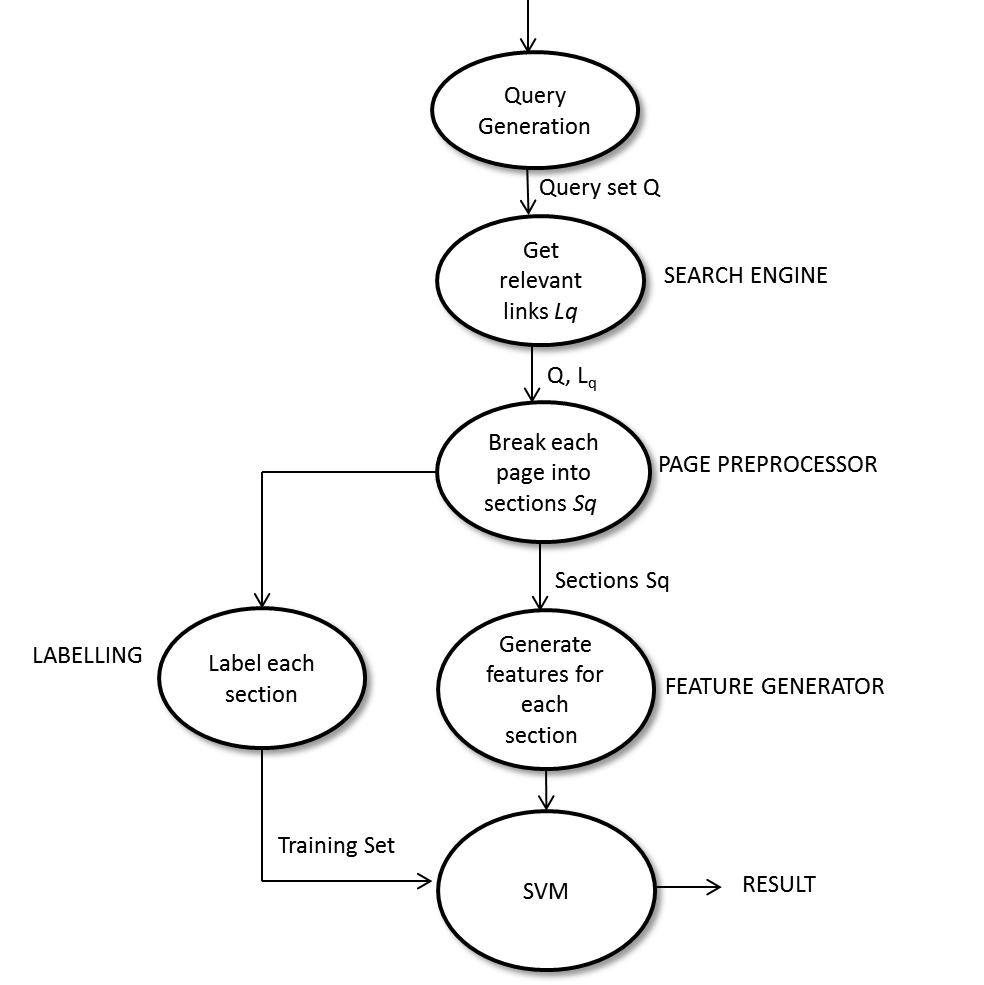
\includegraphics[width=0.6\textwidth]{./diagrams/architecture}\\
\caption{Architecture Diagram}
\end{figure}
\clearpage

\section{Query Generation}

\begin{itemize}

	\item Take the topic $t$ as input.
%	\item Generate set \textbf{T} of related subtopics and add the topic to \textbf{T} as well.
	\item Query Set $Q := T \times \{`questions\textrm', `problems\textrm', `solved\ examples\textrm'\}$.
\end{itemize} 

%Firstly, we will take the input of the topic and generate a list of sub-topics and other keywords which relate to the topic. For eg. if the topic is `Operating Systems', various sub-topics can be `Processes', `Threads', 'Cache' etc. These will form the set \textbf{t}.
\noindent Firstly, we will take the input of the topic $t$.

Topic $t$ will be appended with chosen suffixes such as \emph{`questions'} and \emph{`problems'} to generate the \emph{query set} $Q$ which will be queried on the search engine.

\section{Search Engine}

$\forall q \in Q$ :

\begin{itemize}

	\item Search the internet for the query phrase $q$ using \emph{Google Custom Search API} (or any other search engine).
	\item Add the top \emph{nLinksPerQuery} links to set $L_{q}$.

\end{itemize}

\section{Page Preprocessor}

$\forall l \in$ $L_{q}$ :

\begin{itemize}
	\item Load the link $l$ using \emph{Jsoup} package and use the \emph{HtmlToPlainText} class to strip away all markup data, images etc. and yield only the text portions.
	\item The text of the page is then broken up into \emph{sections} on the basis of --- 
	\begin{itemize}
		\item Number of lines
		\item Paragraph Structure
		\item Interrogative Indicators - \emph{`what', `how', `explain', `define', `?', `elucidate'} etc.
	\end{itemize}
	\item Each \emph{section} $s$ thus obtained is added to the \emph{section set} $S_{q}$.
\end{itemize} 

\noindent For each \emph{query} phrase $q \in Q$, we will load each link we have in our link set $L_{q}$ using \emph{Jsoup} package functions and use the \emph{HtmlToPlainText} class to strip it of all useless markup data, links and pictures and parse out only the text portions available on the page which may contain the questions. 

Each page will then be broken into various \emph{sections}. This will be done by a parser which will determine \emph{sections} which may be questions on the basis of a maximum number of lines, the paragraph tags of html and interrogative indicators like a line ending with a \emph{`?'} or lines starting with words like \emph{`what', `define'} etc. as these are likely to be starting or ending words of a question.

Each \emph{section} $s$ thus obtained will be added to the \emph{section set} $S_{q}$ for a \emph{query}.

\section{Feature Generator}

The feature generator will generate the features and statistics for each \emph{section}, which will be analysed by the SVM to create the regression model. \\

\noindent We adapt the first three features from \emph{SQUINT} to determine the relevance of a \emph{section} to a \emph{query}~\cite{squint}. Furthermore, we propose two additional features to determine whether a \emph{section} contains a question or not. \\

\noindent The features are ---

\subsection {Word Rank Based Features}

The rank of a word is defined to be its position in the list if the words were ordered by frequency of occurrence in \textbf{$S_{q}$}~\cite{squint}. \\

\noindent We would have a feature each for say, the top 200 most frequent words in \textbf{$S_{q}$}. 

For the $i^{th}$ ranked word, this feature would basically have the value for the frequency of this word in the current \emph{section}. \\

\noindent We can limit the dimensionality of the input vector by bucketing words by a certain range of ranks. 
For example, we can bucket ranks 1-5, 6-10, 11-15...etc to aggregate word counts, and come up with a feature vector of reduced dimensionality. 

We also normalize for the length of the \emph{section} since we do not want to be biased towards long \emph{sections}.\\

\noindent The optimal number of words and the bucket size needs to be determined experimentally.

\subsection {Bigram Rank Based Features}

A bigram is defined to be two consecutive words occurring in a \emph{section}~\cite{squint}.\\

\noindent This feature is computed in a manner similar to the previous set of features. \\

\noindent This feature is based on the intuition that the correlation between two words might be more informative than the words taken individually. 

For instance, \emph{`machine learning'} suggests a stronger relation to a query \emph{`AI SVM'} than the
individual words \emph{`machine'} or \emph{`learning'}. \\

\noindent For this feature as well, we will adjust the dimensionality by bucketing and limiting coverage of ranks depending on experimental results.
\clearpage
\subsection {Coverage of Top Ranked Tokens}

Relevance to a topic may also be captured by the coverage of top ranked token types in the \emph{section}~\cite{squint}.\\

\noindent For example, if we have a bucket size of 5, we might be interested in knowing how many of the top 5 ranked words occur in this \emph{section}, how many of the next 5 highly ranked words occur in this \emph{section} and so forth. \\

\noindent For instance, if the top 5 ranked token types are \emph{`learning', `machine', `data', `access', and `database',} and a \emph{section} contains \emph{`learning'} and \emph{`data'}, the corresponding value for this feature is 2.

\subsection {Coverage of Interrogative Indicators}

Presence of words such as \emph{`what', `why', `explain', `define', `elucidate'} etc. are strong indicators that the \emph{section} contains a question. \\

\noindent Thus we propose this feature whose value is the coverage of a predefined set of such interrogative indicators present in the \emph{section}.\\

\noindent We need to experimentally determine whether the frequency or coverage of interrogative indicators is a better feature.

\subsection {Absence of Specific Keywords}

There are certain words or patterns, the presence of which strongly indicate a \emph{section} of text to not have a question. \\

\noindent For example, if a sentence begins with a \emph{`Yes'} or \emph{`No';} or certain words like \emph{`because'} are present, there is a high chance that the \emph{section} is not a question. \\

\noindent We check for the coverage of such words in the \emph{section} using a pre--defined list. 
\clearpage
\section{Labelling (Training Set Generation)}

For generating the training set, we will manually label a set of \emph{sections} as to whether they are relevant questions of the given topic or not and this data will be used to train the SVM to generate the model. 

\section{Support Vector Machine}

This component will be trained using the Training Set comprising of the \emph{section} sets with the generated feature vectors and manually tagged labels. The training data will be analysed to generate a SVM model. \\

\noindent During the real runs of the application, the model generated during training will be used by the SVM to identify the relevant \emph{sections} and tag them appropriately. \\

\noindent The \emph{sections} tagged as \emph{`relevant'} will be added to the result set $R$.

\section{Output}

The output component will take all the \emph{sections} tagged as \emph{`relevant question'} present in set $R$ and output them in a clean format.

\chapter{Prototype}

\emph{Java} was chosen as the programming language owing to the availability of well supported classes to implement SVMs and the object--oriented features in general.\\

\noindent We made a prototype program with placeholder stub functions for each component. Each stub did no useful work but just passed the data along.

Each component would be individually developed and further refined to produce the optimal output.

%---------------------------------------------------

\part{Work Done in S8}

\chapter{Class Design}

The overall design consists of six components. \\

\begin{figure}[h!]
\centering
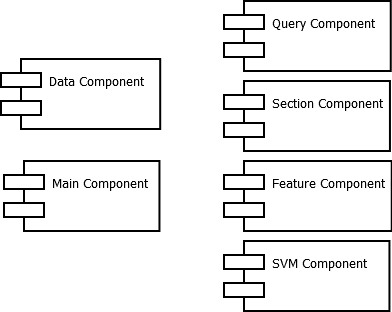
\includegraphics[width=0.50\textwidth]{./diagrams/Component}\\
\caption{Component Diagram}
\end{figure}

\clearpage

%----

\section{Main Component}

This component is responsible for calling all other components and finally generating the list of questions as output. \\

\begin{figure}[h!]
\centering
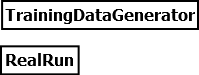
\includegraphics[width=0.25\textwidth]{./diagrams/Main}\\
\caption{Main Component}
\end{figure}

\begin{description}
	\item[TrainingDataGenerator] Calls all components in order and calls the \emph{labeller} so that the training data can be generated.
	\item[RealRun] Once the SVM model is ready, this is used to enter a topic and get list of questions as output.
\end{description}

%-------------------

\section{Data Component}

The \emph{data component} stores the overall data and its classes provide interfaces to access and modify this data. All other components necessarily interact with this component. \\

\begin{figure}[h!]
\centering
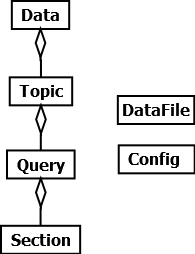
\includegraphics[width=0.30\textwidth]{./diagrams/Data}\\
\caption{Data Component}
\end{figure}

\begin{description}
	\item[DataFile] Interface to the data file.
	\item[Config] Has all the config parameters as set in \emph{config.properties} file.
    \item[Data] Stores a list of \emph{topic objects}.
    \item[Topic] Stores the input topic and a list of \emph{query objects}.
	\item[Query] Stores the details related to each \emph{query}. Has a list of associated \emph{section objects}.
	\item[Section] Stores the \emph{section} text and relevant attributes.
\end{description}

\clearpage

%----

\section{Query Component}

The \emph{query component} is responsible for taking the input topic and generating queries related to the same. \\
\begin{figure}[h!]
\centering

\includegraphics[width=0.50\textwidth]{./diagrams/Query}\\
\caption{Query Component}
\end{figure}

\begin{description}
	\item[TopicListGenerator] Generates a list of related and/or sub--topics related to the input.
	\item[QueryGenerator] Generates list of \emph{query objects} by adding various suffixes to the given topic.
\end{description}

%----

\section{Section Component}

The \emph{section component} processes each \emph{query} and generates a list of \emph{section objects} for each \emph{query}. \\

\begin{figure}[h!]
\centering

\includegraphics[width=0.70\textwidth]{./diagrams/Section}\\
\caption{Section Component}
\end{figure}

\begin{description}
	\item[LinkGenerator] Uses a Search API to search for the \emph{query} and generate links of the top results.
	\item[HTMLParser] Uses the \emph{JSoup} package to load links and return plaintext form of the web--pages.
	\item[SectionGenerator] Breaks pages into sections and makes a \emph{section object} for each.
\end{description}

\clearpage

%----

\section{Feature Component}

The \emph{feature component} has classes to generate all the requisite features for the \emph{sections}. \\

\begin{figure}[h!]
\centering
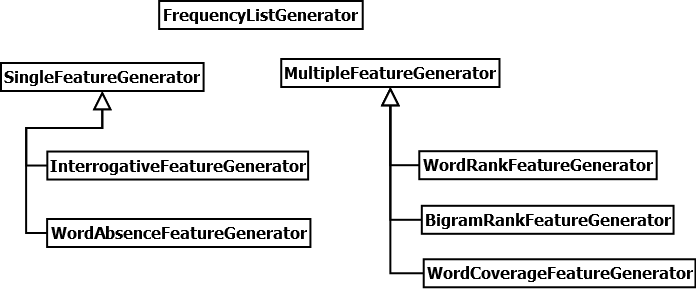
\includegraphics[width=0.90\textwidth]{./diagrams/Feature}\\
\caption{Feature Component}
\end{figure}

\begin{description}
	\item[FrequencyListGenerator] Processes all the \emph{sections} related to a \emph{query} to generate a list of words and bigrams in descending order of frequency.
	\item[SingleFeatureGenerator] Interface for feature--types that generate a single feature.
	\item[MultipleFeatureGenerator] Interface for feature--types that generate a list of features.
	\item[WordRankFeatureGenerator] Generates the Word Rank based feature list of the \emph{section}.
	\item[BigramRankFeatureGenerator] Generates the Bigram Rank based feature list of the \emph{section}.
	\item[WordCoverageFeatureGenerator] Generates the Word Coverage based feature list of the \emph{section}.
	\item[InterrogativeFeatureGenerator] Generates the Interrogative Indicator frequency based feature of the \emph{section}.
	\item[WordAbsenceFeatureGenerator] Generates the feature based on absence of specific words of the \emph{section}.
\end{description}

\clearpage

%----

\section{SVM Component}

Consists of all the classes which are related to the machine learning aspect of the program. \\

\begin{figure}[h!]
\centering
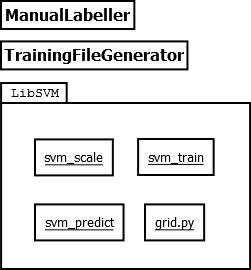
\includegraphics[width=0.40\textwidth]{./diagrams/SVM}\\
\caption{SVM Component}
\end{figure}

\begin{description}
	\item[ManualLabeller] Loads each \emph{section} one by one and allows the user to manually label the \emph{sections}.
    \item[TrainingFileGenerator] Generates the Training File with all labels and features in the correct format.
	\item[LibSVM] The Support Vector Machine library. It consists of the following ---
\begin{description}
        \item[svm\_scale] Scales the training file features.
        \item[svm\_train] Trains the SVM and generates the model file.
        \item[svm\_predict] Predicts the output as per model file for a data file.
        \item[grid.py] Python script to determine best C\footnote{The SVM parameter C trades off misclassification of training examples against simplicity of the decision surface~\cite{params}.} and $\gamma$\footnote{The RBF Kernel parameter $\gamma$ defines how far the influence of a single training example reaches~\cite{params}.} values for the SVM.
    \end{description}
\end{description}

\clearpage

%--------------------------------------------------

\chapter{Data Structure Design}

We have chosen to use an n--ary tree as the data structure keeping in mind the component--based architecture. \\

The tree structure allows us to model the data easily while being completely extensible at any point. 
It allows quick access to required data and allows us to group data in a functional manner. 

\section{Node Design}

The node will have the following attributes : 
\begin{description}
	\item[Type] The type of the node eg. \emph{Topic}, \emph{Query}, \emph{Section}
	\item[Data] The corresponding data eg.\emph{ `SVM Questions'}
	\item[ChildList] List of child nodes
\end{description}

\begin{figure}[h!]
\centering
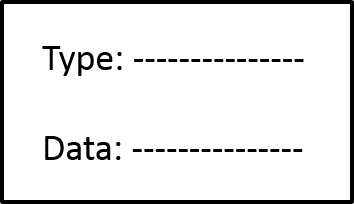
\includegraphics[width=0.30\textwidth]{./diagrams/node}\\
\caption{Node}
\end{figure}

\clearpage 

\section{Tree Design}

The tree will look like the following --- \\

\begin{figure}[h!]
\centering
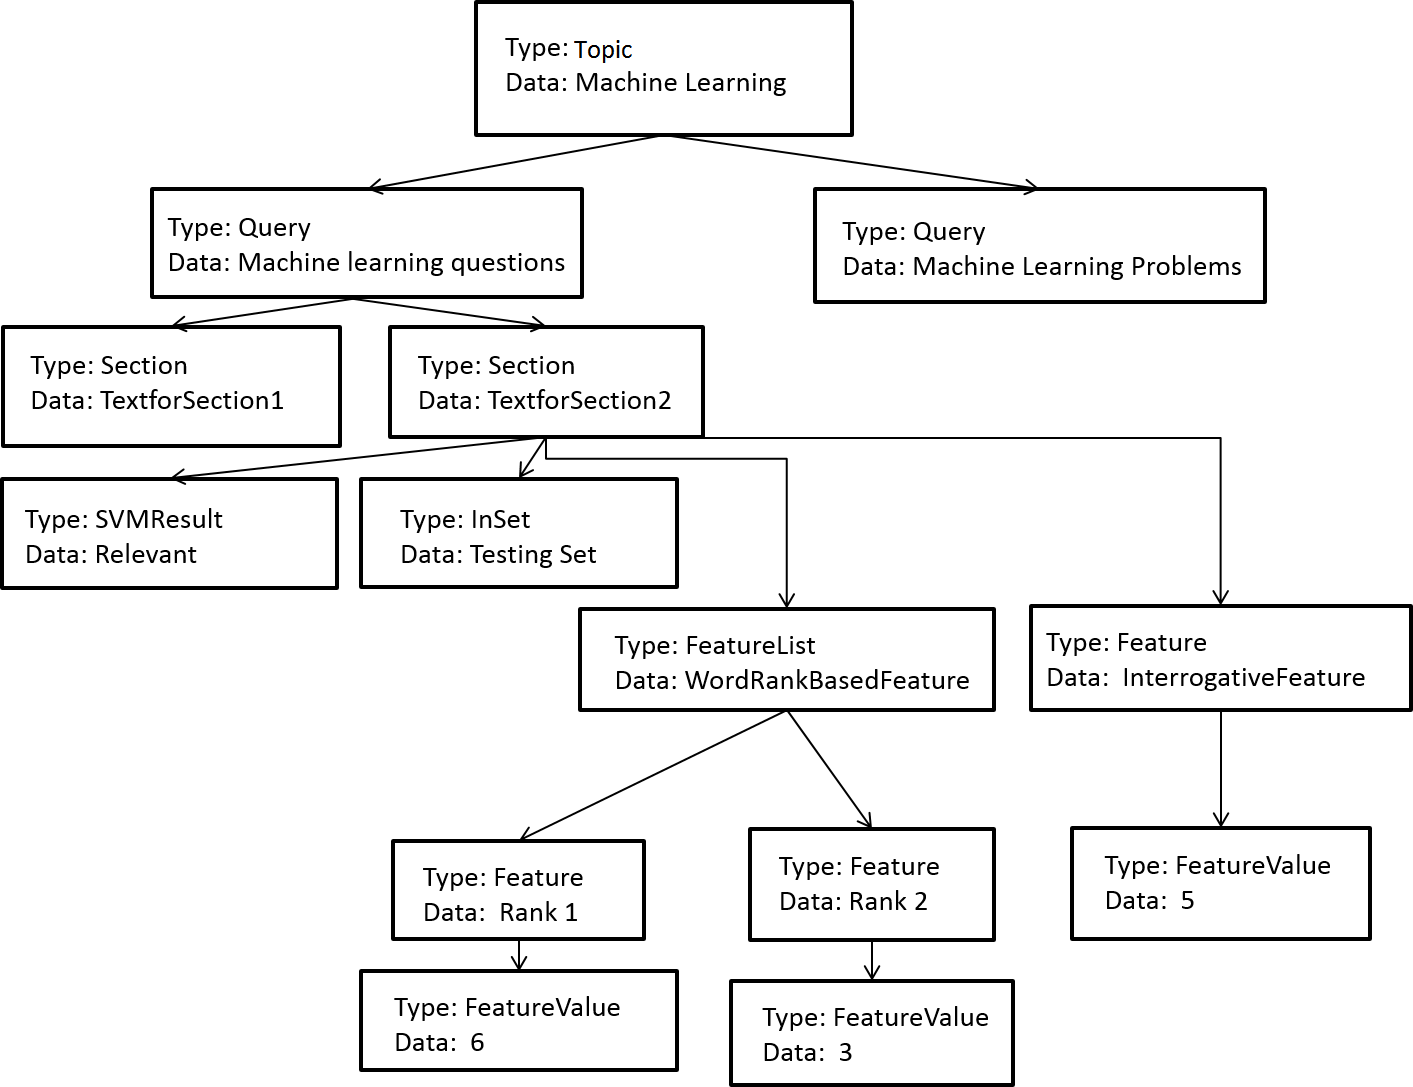
\includegraphics[width=\textwidth]{./diagrams/tree}\\
\caption{The data tree}
\end{figure}

Each node will have its corresponding data in its child nodes. \\

As each component is run, it will add or delete nodes as required. \\

\clearpage
\section*{The Data Tree Life--Cycle}

\subsection{Query Generation}

The Query Generator generates a set of \emph{queries} to search for from the given search \emph{topic} and creates a set of corresponding nodes as children to the root node, as shown.

\begin{figure}[h!]
\centering
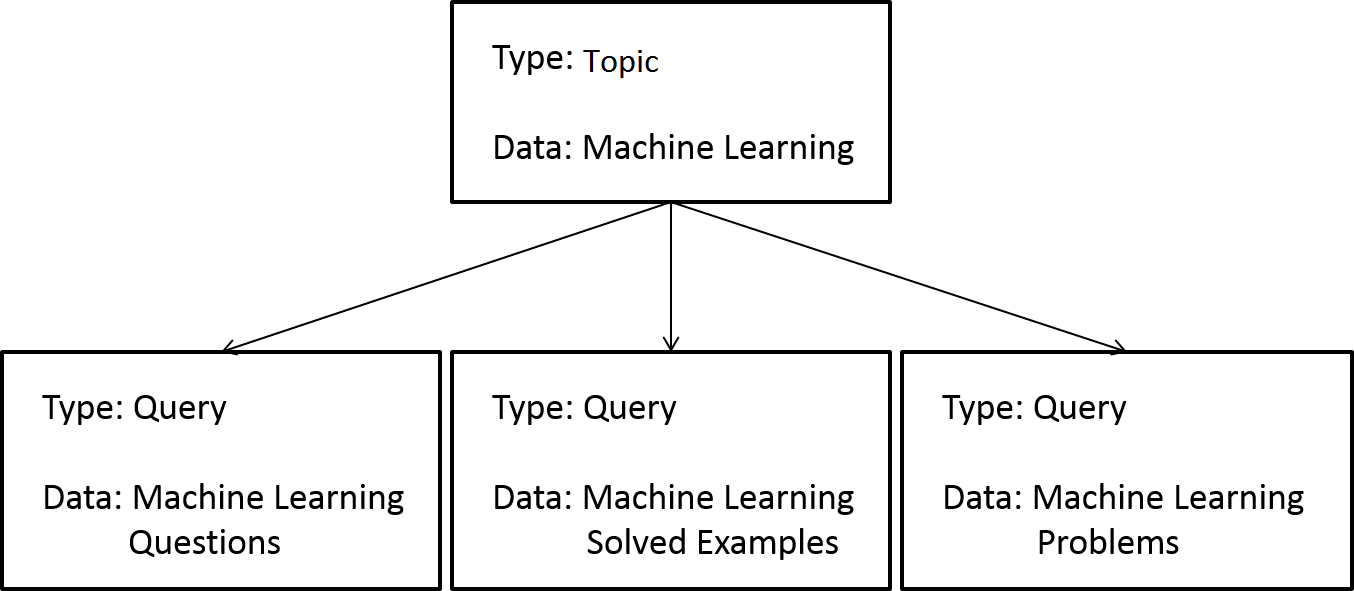
\includegraphics[width=0.80\textwidth]{./diagrams/tree1}\\
\caption{Query Generation Data}
\end{figure}

\subsection{Link Generation}

For each of the \emph{queries} generated in the previous step, a set of links corresponding to the search results for that \emph{query} is generated as children of each \emph{query} node. 

\begin{figure}[h!]
\centering
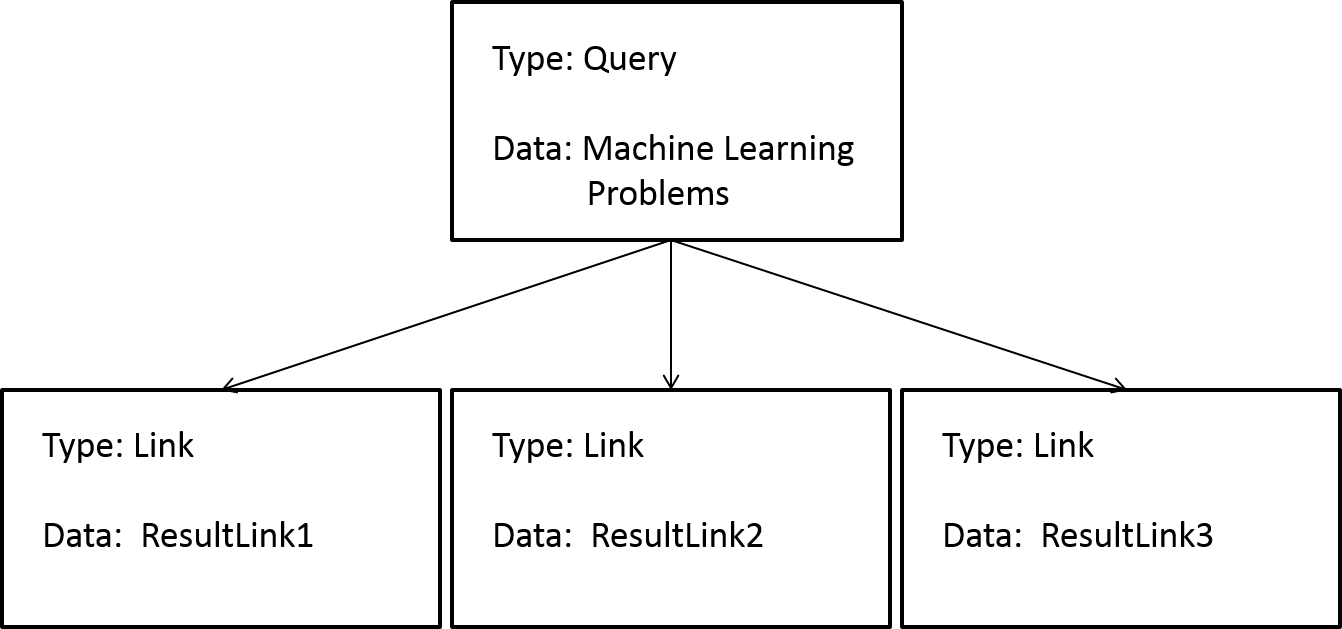
\includegraphics[width=0.80\textwidth]{./diagrams/tree2}\\
\caption{Link Generation Data}
\end{figure}

\clearpage

\subsection{Section Generation}

The \emph{Section Generator} parses each of the links generated in the previous step, removing unnecessary data and then divides each such page into \emph{sections}, each of which may contain a question relevant to the topic at hand. 

\begin{figure}[h!]
\centering
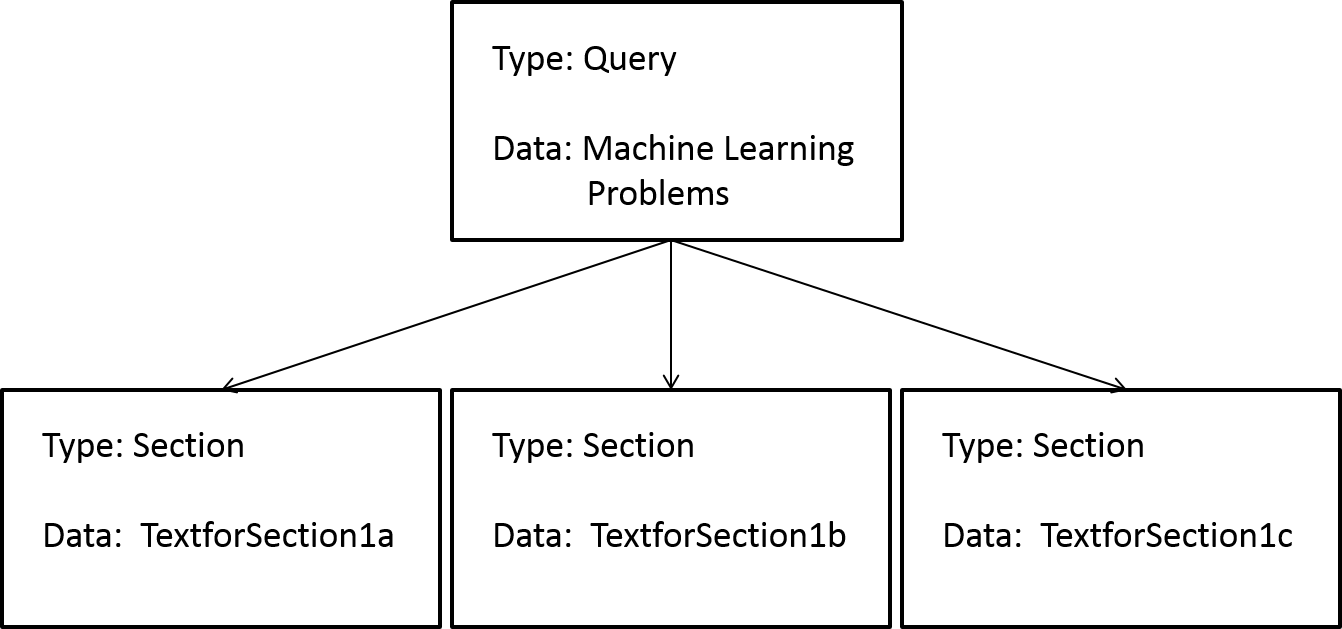
\includegraphics[width=0.80\textwidth]{./diagrams/tree3}\\
\caption{Section Generation Data}
\end{figure}

\subsection{Labelling}

\emph{Sections} intended to be part of the training or testing set will be labelled as relevant or not relevant. This is indicated by a corresponding child node for that \emph{section} node, as shown.

\begin{figure}[h!]
\centering
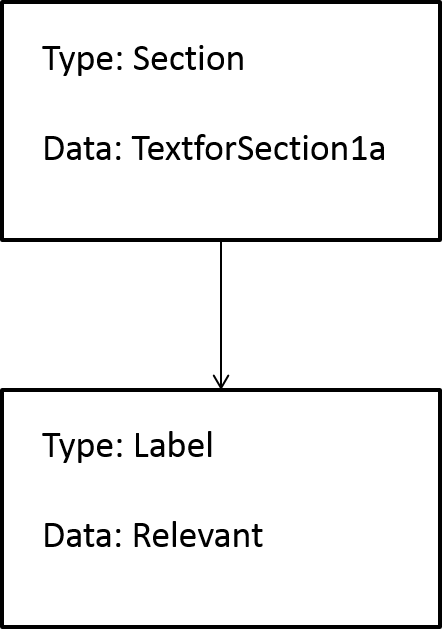
\includegraphics[width=0.30\textwidth]{./diagrams/tree4}\\
\caption{Labelling Data}
\end{figure}

\clearpage

\subsection{Feature Generation}

The features of a \emph{section} are similarly represented by corresponding child nodes of each feature category. 

\begin{figure}[h!]
\centering
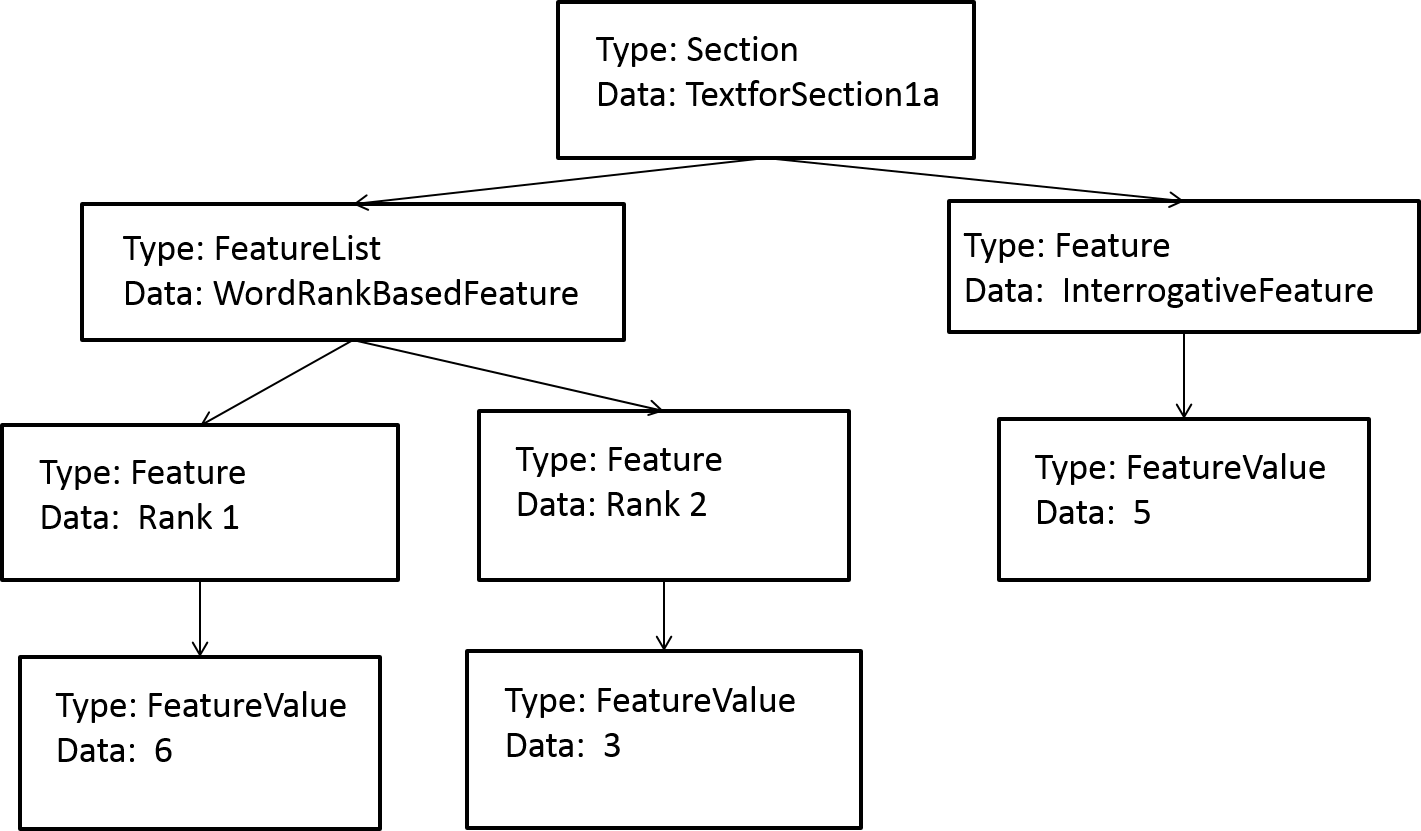
\includegraphics[width=0.80\textwidth]{./diagrams/tree5}\\
\caption{Feature Data}
\end{figure}

\subsection{SVM Classification}

The results of the Support Vector Machine classification and the set to which the result belongs are also represented as shown. 

\begin{figure}[h!]
\centering
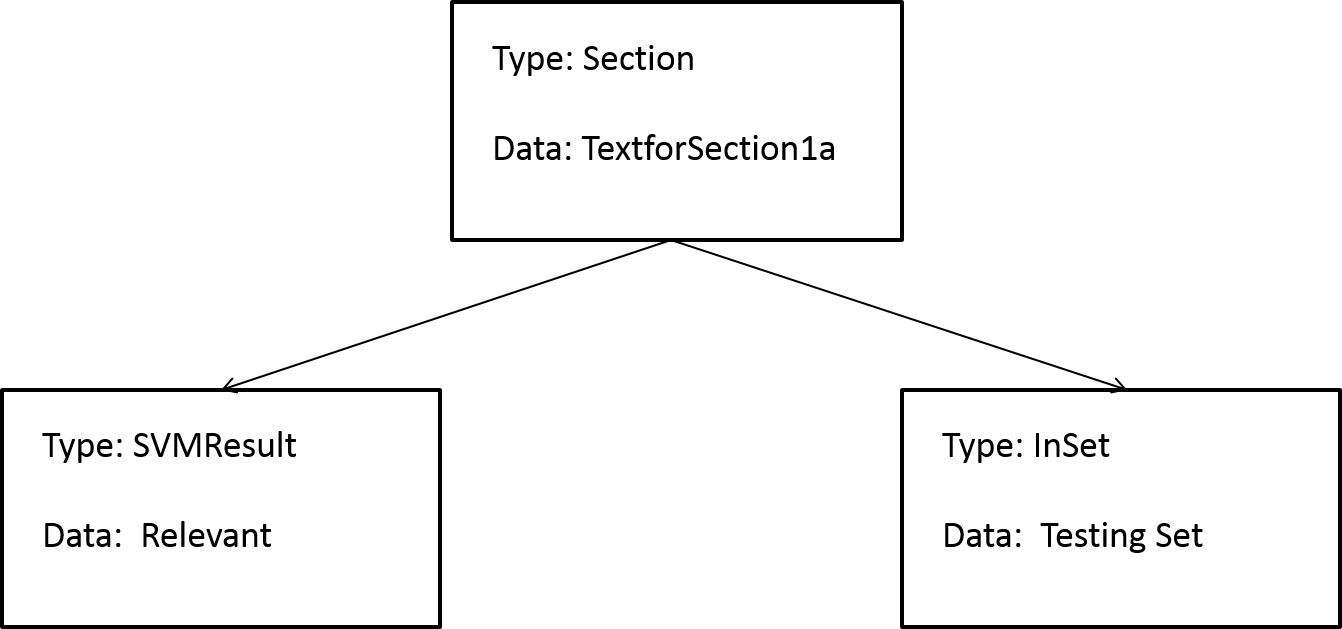
\includegraphics[width=0.80\textwidth]{./diagrams/tree6}\\
\caption{SVM Data}
\end{figure}

\clearpage

%---------------------------------------------

\chapter{Data File Design}

We will be using the \emph{XML} file format for the data file since the tree--like structure of the \emph{XML} format is highly suitable for representing a tree data structure~\cite{wikixml}. \\

\noindent The file, \emph{data.xml}, will be a representation of the data stored in a tree format. \\

\noindent Each node of the tree will be represented as an element\footnote{A logical document component which either begins with a start-tag and ends with a matching end-tag. The characters between the start- and end-tags, if any, are the element's content and may contain other elements, which are called child elements. Eg. \textless Type\textgreater Data\textless \textbackslash Type\textgreater.} in the \emph{XML} file delineated by the tags of the node--type. 
Each child--node in the tree will be represented as child--elements of the corresponding parent node. \\

\noindent The key features of this design are its performance, extensibility and transparent nature which allows us to analyse the file at any point in the application's life--cycle. \\

\noindent The Java \emph{JAXB}\footnote{\emph{Java Architecture for XML Bindings} is capable of writing/reading annotated object data to/from an \emph{XML} file.} feature is capable of loading the data from the file directly into a tree format as per the class definitions. This will allow us to easily read, write or update the data file as required.

\begin{figure}[h!]
\centering
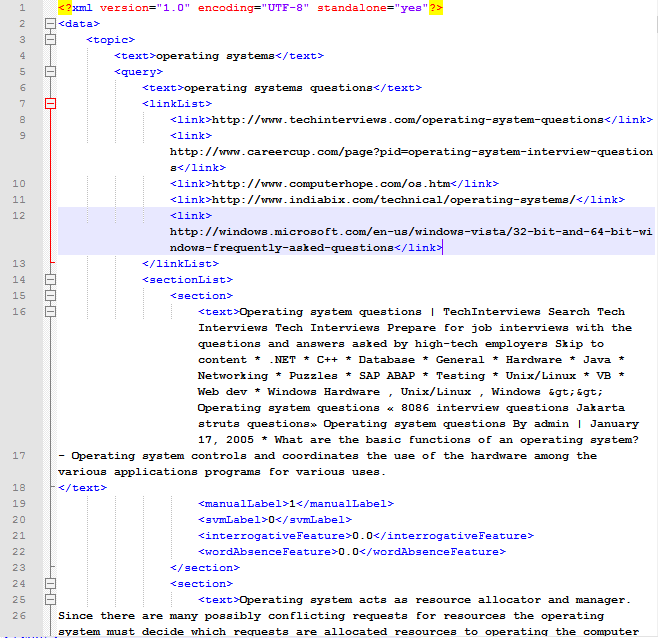
\includegraphics[width=\textwidth]{./diagrams/xml}\\
\caption{data.xml example}
\end{figure}

\clearpage

%---------------------------------------------

\chapter{Config File Design}

The file \emph{config.properties} will have all the configurable parameters in the Java \emph{Properties} format. \\

\noindent The values will be loaded from this file every time the application runs. Thus we need not re--compile the entire application just to change the parameters. \\

\noindent The parameters can be changed in a simple manner using any text--editor. \\

\noindent Thus the user is free to change the parameters as per his/her requirements. 

This will help reduce wastage of time during testing and analysis of parameters by eliminating needless re-compilations.

\begin{figure}[h!]
\centering
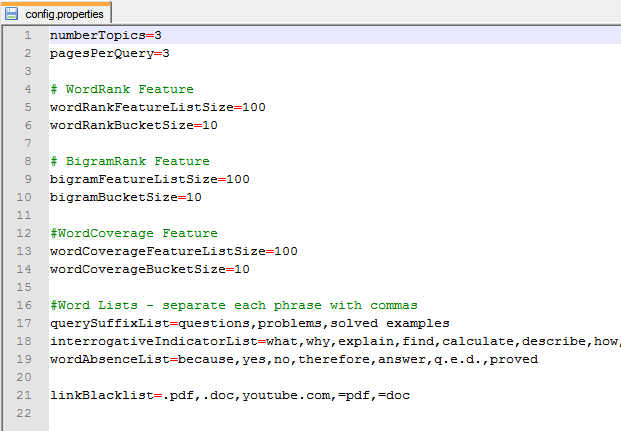
\includegraphics[width=\textwidth]{./diagrams/config}\\
\caption{config.properties}
\end{figure}

\clearpage

%---------------------------------------------

\chapter{SVM Package Identification}

We have identified the \emph{LIBSVM}~\cite{libsvm} library to implement the Support Vector Machine. \\

\noindent We are using \emph{LIBSVM} because it has functions for the \emph{Radial Basis Kernel}~\cite{libsvmpaper}. 

This kernel nonlinearly maps samples into a higher dimensional space so it, unlike the linear kernel, can handle the case when the relation between class labels and attributes is nonlinear~\cite{libsvmpaper}.\\

\noindent \emph{LIBSVM} is a mature SVM library for Java and has good performance and high accuracy~\cite{libsvmpaper}.

%---------------------------------------------

\chapter{Section Generation Heuristic}

Paragraph and sentence boundary detection is done using the \emph{SentParDetector} class from the \emph{Spiatools} library by Scott Piao~\cite{spiatools}. 

It is a highly accurate sentence and paragraph breaker, employing heuristic rules for identifying boundaries. \\

\noindent Sentences returned by the \emph{SentParDetector} class having length more than 400 characters are again attempted to be broken 
down using the standard \emph{BreakIterator} class provided by Java.  \\

\noindent As questions are likely to be contained in fewer than four sentences, every paragraph returned by the \emph{SentParDetector}
class containing six or more sentences is broken up into half, and the check is repeated on the individual paragraphs too.

%---------------------------------------------

\chapter{Frequency List Generation}

The \emph{FrequencyListGenerator} class generates bigram and unigram word frequencies for \emph{query objects} and \emph{section objects}. \\

\noindent The text content from the corresponding \emph{object} is broken into tokens using the \emph{StandardTokenizer} class from the \emph{Apache Lucene} library~\cite{apachelucene}. 
\emph{StandardTokenizer} is a grammar--based tokenizer constructed with \emph{JFlex}~\cite{jflex}. 
This class implements the \emph{Word Break} rules from the\emph{ Unicode Text Segmentation} algorithm, as specified in Unicode Standard Annex \#29~\cite{unicode}.

\section{Unigram Frequency Generation}

The tokens generated by the \emph{StandardTokenizer} are iterated over. Each token is mapped to a hashtable using the token string 
as the key, and setting the frequency of occurrence of the token in the text as the hash value. 
The hashmap is sorted in the decreasing order of token frequencies, and the corresponding \emph{object} word frequency list is set as this hashmap.

\section{Bigram Frequency Generation}

\emph{ShingleFilter} class from \emph{Apache Lucene} library helps in constructing shingles (token n--grams) from a token stream. 
The bigram frequency generator uses the \emph{ShingleFilter} class to generate bigram tokens from the tokens generated by the \emph{StandardTokenizer}.
These bigram tokens are then mapped to a hashtable in a similar manner to unigram frequency generation to obtain bigram token frequencies, and this hashmap is set as the bigram frequency list of the corresponding \emph{object}.

%---------------------------------------------

\chapter{Implementation and Analysis}

The entire program was successfully implemented in Java as per the proposed design.

\section{Training Data Generation}

The Training Data was generated by running \emph{EQML1} for 3 topics --- \emph{`operating systems', `data structures and algorithms', `computer architecture'}. 
This resulted in a total of $6467$ \emph{sections} being generated which were saved in \emph{data.xml}.

\begin{itemize}
\item $5223$ \emph{sections} were marked irrelevant.
\item $1243$ \emph{sections} were marked relevant.
\end{itemize}

\noindent \emph{EQML2} was used to generate the SVM Feature files by first loading the \emph{data.xml} file and then calculate the features based on various combinations of the configurable parameters.

Since we have 4 times the number of irrelevant \emph{sections} vs. relevant \emph{sections}, we use a weightage of 4 for relevant \emph{sections} and weightage of 1 for irrelevant \emph{sections} while training the SVM to avoid unbalanced data bias~\cite{weightedsvm}.
\clearpage
\section{Performance Measure}

Let $x_1,x_2,...,x_n$ be the testing data and $f(x_1),f(x_2),...,f(x_n)$ be the decision values by the SVM. If true labels (manual labels) are denoted by $y_1,y_2,...,y_n$ then accuracy can be thought of as the percentage of correctly predicted data vs. the total testing data~\cite{libsvmpaper}.
\[ t_i = \left\{
	\begin{array}{ll}
		1 & \mbox{if } f(x_i) = y_i \\
		0 & \mbox{if } f(x_i) \neq y_i 
	\end{array}
\right. \]


\[ Accuracy = \frac{\sum t_i}{n} \times 100\% \]

\noindent Cross--validation is a model validation technique for assessing how the results of a statistical analysis will generalize to an independent data set~\cite{crossvalidation}. 

It is mainly used in settings where the goal is prediction, and one wants to estimate how accurately a predictive model will perform in practice. 

Cross-validation is important in guarding against testing hypotheses suggested by the data \emph{(``Type III errors")}~\cite{crossvalidation}.\\

\noindent In \emph{k-fold cross-validation}, the original sample is randomly partitioned into $k$ equal size subsamples. 
Of the $k$ subsamples, a single subsample is retained as the validation data for testing the model, 
and the remaining $k - 1$ subsamples are used as training data. The cross-validation process is then repeated k times (the folds), 
with each of the $k$ subsamples used exactly once as the validation data. The $k$ results from the folds then can be averaged
to produce a single estimation. 

The advantage of this method over repeated random sub-sampling is that all observations are 
used for both training and validation, and each observation is used for validation exactly once~\cite{crossvalidation}.\\

\noindent \emph{5--fold Cross Validation Accuracy} was chosen as the performance measure.
\clearpage
\section{Feature Analysis}

\subsection{Procedure}

For each configuration of features ---
\begin{enumerate}
    \item Features were generated by configuring the \emph{config.properties} file
    \item The features were scaled\footnote{Scaling is done to avoid the problem of features having greater numeric range dominating the results~\cite{libsvmppt}.} to $[0,1]$ using svm\_scale
    \item Optimal $C$ and $\gamma$ SVM parameters were determined using \emph{grid.py}
    \item \emph{5--fold Cross Validation Accuracy} was determined
\end{enumerate}
\clearpage
\subsection{Observations}

\subsubsection{Word Rank Based Features}

The Word Rank Feature set size was varied while keeping the other features constant.

\begin{itemize}
\item Word Rank Bucket Size = 1
\item Bigram Rank Features = 150
\item Bigram Rank Bucket Size = 1
\item Word Coverage Based Features = 150
\item Word Coverage Bucket Size = 5
\end{itemize}

\begin{figure}[h!]
\centering
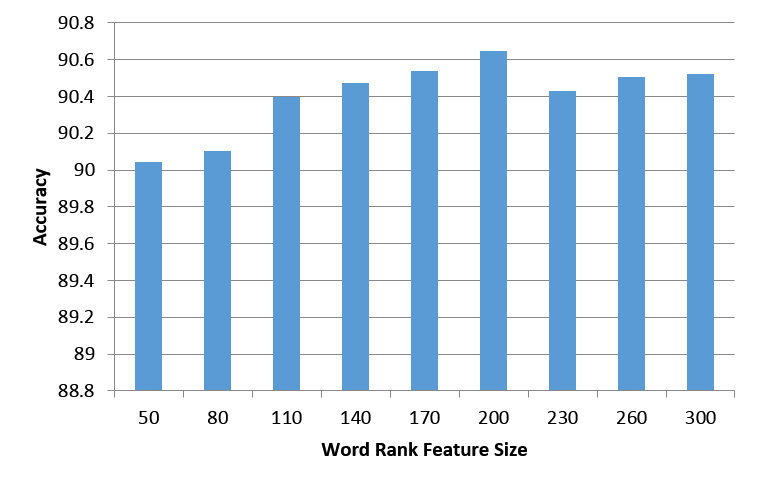
\includegraphics[width=\textwidth]{./diagrams/wrf}\\
\caption{Word Rank Features}
\end{figure}

\noindent The accuracy increased with the set size upto a point and then varied. This leads us to believe that the first 150 word ranks are significant beyond which the data becomes less relevant.

%----
\clearpage
\subsubsection{Bigram Rank Based Features}

The Bigram Rank Feature set size was varied while keeping the other features constant.

\begin{itemize}
\item Word Rank Features = 150
\item Word Rank Bucket Size = 1
\item Bigram Rank Bucket Size = 1
\item Word Coverage Based Features = 150
\item Word Coverage Bucket Size = 5
\end{itemize}

\begin{figure}[h!]
\centering
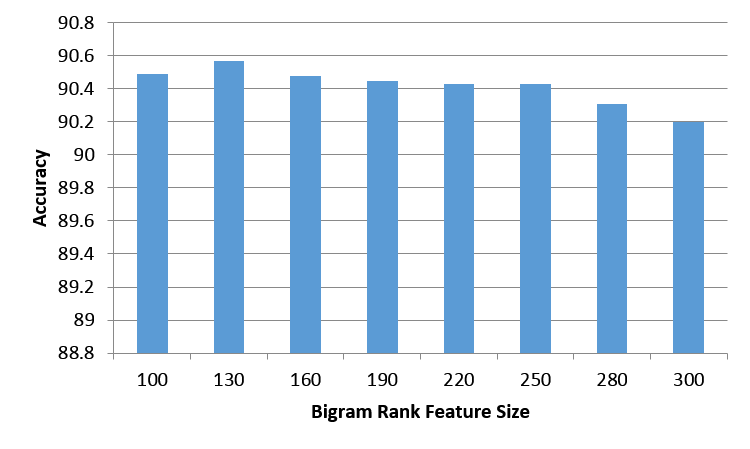
\includegraphics[width=\textwidth]{./diagrams/brf}\\
\caption{Bigram Rank Features}
\end{figure}

\noindent The accuracy was higher around the 130--150 mark but beyond that the accuracy dropped. This is probably due to the first few bigrams capturing data about the topic but beyond that random bigrams make the data too noisy to matter.

%---
\clearpage
\subsubsection{Word Coverage Based Features}

The Word Coverage Feature set size was varied while keeping the other features constant.

\begin{itemize}
\item Word Rank Features = 150
\item Word Rank Bucket Size = 1
\item Bigram Rank Features = 150
\item Bigram Rank Bucket Size = 1
\item Word Coverage Bucket Size = 5
\end{itemize}

\begin{figure}[h!]
\centering
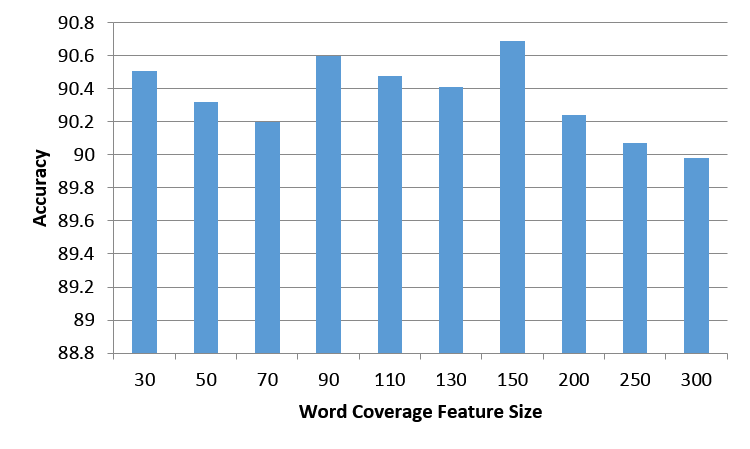
\includegraphics[width=\textwidth]{./diagrams/wcf}\\
\caption{Word Coverage Features}
\end{figure}

\noindent There was significant variation in accuracy as the number of features changed. The maximum accuracy was observed at 150 features.

\clearpage

\subsubsection{Optimal Feature Configuration}

Based on the insights obtained, all the features were varied and the optimal accuracy was determined.

\begin{figure}[h!]
\centering
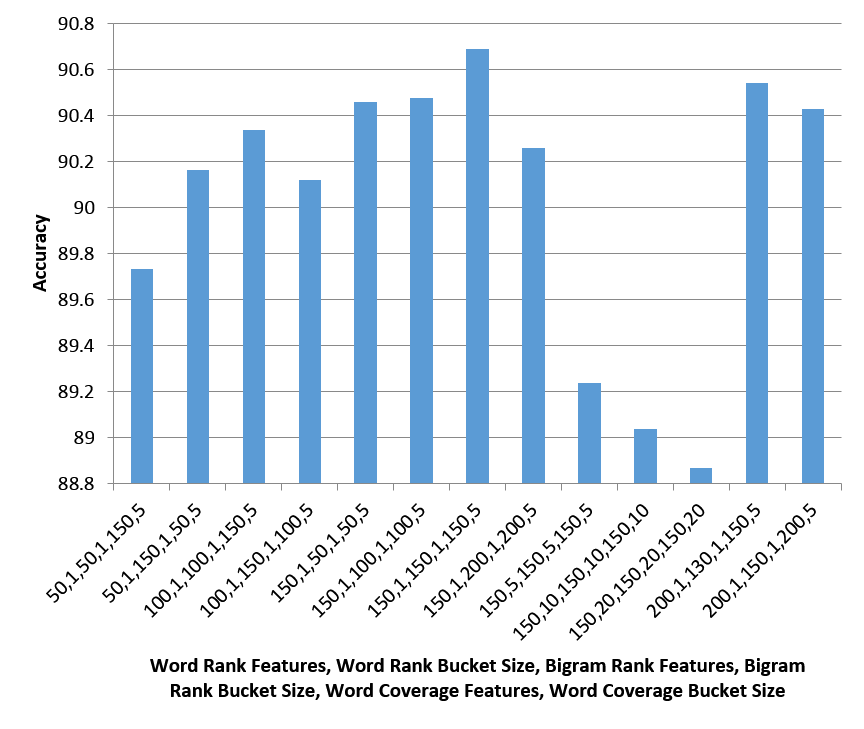
\includegraphics[width=\textwidth]{./diagrams/optimal}\\
\caption{Optimal Feature Configuration Detection}
\end{figure}

\paragraph{Optimal Configuration --- Accuracy 90.69\%}
\begin{itemize}
\item Word Rank Features = 150
\item Word Rank Bucket Size = 1
\item Bigram Rank Features = 150
\item Bigram Rank Bucket Size = 1
\item Word Coverage Features = 150
\item Word Coverage Bucket Size = 5
\end{itemize}

\paragraph{Optimal SVM parameters}
\begin{itemize}
\item $C = 8.0$
\item $\gamma = 0.125$
\end{itemize}
This feature set was used to generate the model for the Real Run.
\clearpage
\section{Training Set Size Analysis}

\subsection{Procedure}

The effect of Training Set size on the accuracy was determined by ---
\begin{enumerate}
\item Training Set was generated using stratified subsampling\footnote{Stratified sampling using proportionate allocation uses a sampling fraction in each of the 
strata that is proportional to that of the total population. For instance, if the population consists 
of 60\% in the male stratum and 40\% in the female stratum, then the relative size of the two samples (three males, two females) should reflect this proportion~\cite{stratified}.} 
of the Data Set
\item The features were scaled\footnote{Scaling is done to avoid the problem of features having greater numeric range dominating the results~\cite{libsvmppt}.} to $[0,1]$ using \emph{svm\_scale}
\item Optimal $C$ and $\gamma$ SVM parameters were determined using \emph{grid.py}
\item SVM Model was generated using the Training Set
\item Accuracy was calculated by predicting the Data Set
\end{enumerate}

\noindent The optimal feature configuration determined earlier was used for this analysis. 

\subsection{Observation}

We see that the accuracy increases exponentially with training set size. 

\begin{figure}[h!]
\centering
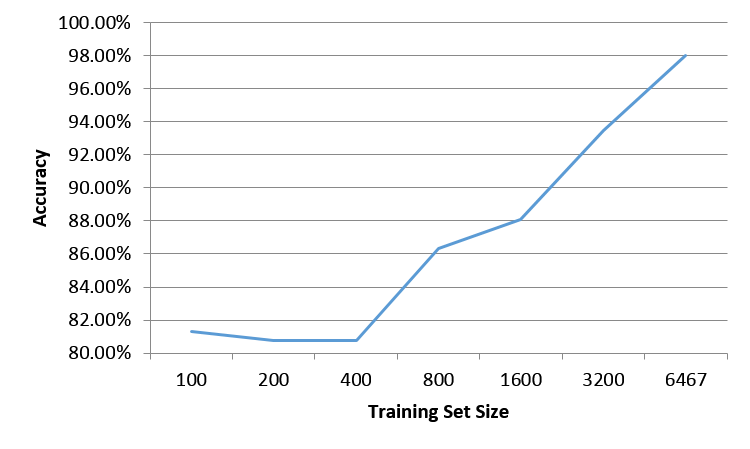
\includegraphics[width=\textwidth]{./diagrams/setsize}\\
\caption{Learning Curve}
\end{figure}

\noindent Thus we choose to make the final model with the full $6467$ samples as the Training Set. 

Higher number of samples is avoided to keep the training time low as training time is proportional to $(SetSize)^2$~\cite{libsvmpaper} and to avoid the problem of over--fitting\footnote{Overfitting occurs when a statistical model describes random error or noise instead of the underlying relationship. Overfitting generally occurs when a model is excessively complex, such as having too many parameters relative to the number of observations. A model which has been overfit will generally have poor predictive performance, as it can exaggerate minor fluctuations in the data~\cite{overfitting}.}.

\section{Proposed Features Analysis}

\subsection{Procedure}

The effect of our proposed features was studied by ---
\begin{enumerate}
    \item Configurations of the Training File were generated by selecting combinations of the 3 classes\footnote{Interrogative Features, Word Absence Features and \emph{SQUINT} Features} of features\footnote{The trivial case with no features was discarded}
    \item The features were scaled\footnote{Scaling is done to avoid the problem of features having greater numeric range dominating the results~\cite{libsvmppt}.} to $[0,1]$ using \emph{svm\_scale}
    \item Optimal $C$ and $\gamma$ SVM parameters were determined using \emph{grid.py}
    \item \emph{5--fold Cross Validation Accuracy} was determined
\end{enumerate}

\subsection{Observation}

The Interrogative feature succeeds in identifying whether a \emph{section} is a question but is not capable of determining irrelevant questions by itself. 

Using the Interrogative feature with the \emph{SQUINT} features results in a $90.55\%$ accuracy and adding the Word Absence features results in accuracy of $90.69\%$.

\begin{figure}[h!]
\centering
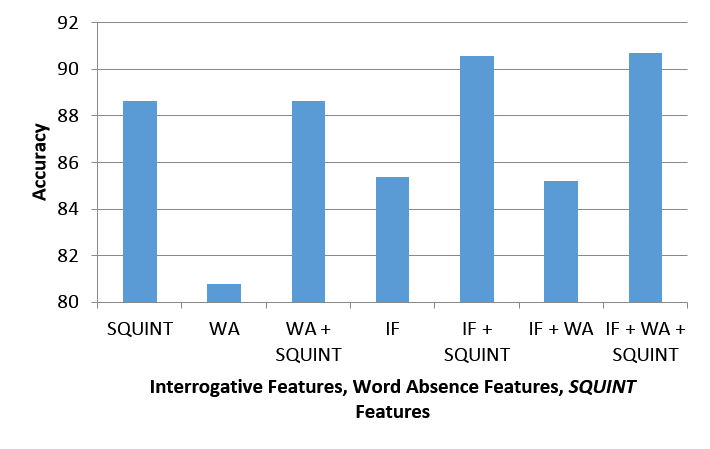
\includegraphics[width=\textwidth]{./diagrams/ourfeatures}\\
\caption{Proposed Features}
\end{figure}

\noindent Thus it is optimal to use all the features.
\clearpage

\section{Real Run}

On giving a topic as input, the program searches the web for relevant pages, retrieves these pages, breaks them into \emph{sections}, generates the requisite features and then the \emph{svm\_predict} module is called to get the predictions of whether the \emph{sections} are relevant or not. \\

\noindent The SVM uses the optimal model generated using our manually labelled data with the optimal feature set.\\

\noindent The \emph{sections} which are predicted to be relevant are stored in a file, \emph{realOutput.txt}, as output and this contains the required list of questions relevant to the topic given as input.

\begin{figure}[h!]
\centering
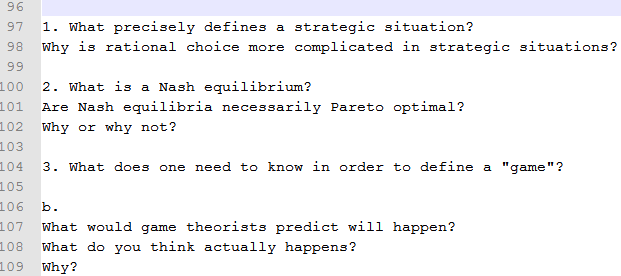
\includegraphics[width=\textwidth]{./diagrams/realrun}\\
\caption{Sample Output for Topic -- Game Theory}
\end{figure}

%---------------------------------------------------

\chapter{Conclusion and Future Work}

Our proposed method of using a SVM to classify relevant questions from the internet seems successful. \\

\noindent Future work may comprise of using different types of classifiers for the Machine Learning component like Neural Networks. \\

\noindent Our solution discards the information when a \emph{section} is relevant to the topic but is not a question as it is marked as not--relevant. 
A multi--class SVM classification approach may be used to capture this data into four classes --- Not~Relevant~Not~Question, Not~Relevant~Question, Relevant~Not~Question, Relevant~Question.\\

\noindent Other features to better analyse whether a \emph{section} is a question or not may also be explored to improve the accuracy of the classification.

%------------------------------------------------------------------------

\clearpage
\addcontentsline{toc}{chapter}{References}
\begin{thebibliography}{99}

\bibitem{squint} SQUINT - SVM for Identification of Relevant Sections in Web Pages for Web Search, \textbf{Riku Inoue, Siddharth Jonathan J.B., Jyotika Prasad}, \emph{Department of Computer Science, Stanford University}

\bibitem{teevan} The Perfect Search Engine is Not Enough : A Study of Orienteering Behavior in Directed Search, \textbf{Jaime Teevan, Christine Alvarado, Mark S. Ackerman and David R. Karger}, \emph{Proceedings of the SIGCHI conference on Human factors in computing systems. pp. 415-422, April 2004.}

\bibitem{wikiML} Wikipedia article on Machine Learning, \url{http://en.wikipedia.org/wiki/Machine_learning}

\bibitem{elements} The Elements of Statistical Learning: Data Mining, Inference, and Prediction, \textbf{Trevor Hastie, Robert Tibshirani, Jerome Friedman}

\bibitem{joachims} Text Categorization with Support Vector Machines: Learning with Many Relevant Features, \textbf{Thorsten Joachims}, \emph{Universitat Dortmund, Informatik LS8, Baroper Str. 301, 44421 Dortmund, Germany}

\bibitem{wikiSVM} Wikipedia article on Support Vector Machine, \url{http://en.wikipedia.org/wiki/Support_vector_machine}

\bibitem{wiki} Machine Learning, \url{http://en.wikipedia.org/wiki/Machine_Learning}

\bibitem{coursera} Machine Learning Course on Coursera, \url{https://class.coursera.org/ml-2012-002/class/index}

\bibitem{wikixml} XML, \url{http://en.wikipedia.org/wiki/XML}

\bibitem{libsvm} LIBSVM, \url{http://www.csie.ntu.edu.tw/~cjlin/libsvm/}

\bibitem{libsvmpaper} LIBSVM, \textbf{Chih-Wei Hsu, Chih-Chung Chang, and Chih-Jen Lin}, April 15, 2010.

\bibitem{libsvmppt} A Practical Guide to Support Vector Classification, \textbf{Chih-Jen Lin}, \emph{Department of Computer Science, National Taiwan University}, \emph{Talk at University of Freiburg},\emph{ July 15, 2003.}

\bibitem{weightedsvm} An approach for classification of highly imbalanced data using weighting and undersampling, \textbf{Ashish Anand, Ganesan Pugalenthi, Gary B. Fogel, P. N. Suganthan}, \emph{Springer Journal}.

\bibitem{params} RBF SVM Parameters, \url{http://scikit-learn.org/dev/auto_examples/svm/plot_rbf_parameters.html}

\bibitem{crossvalidation} Cross-validation (statistics), \url{http://en.wikipedia.org/wiki/Cross-validation_(statistics)}

\bibitem{apachelucene} Apache Lucene --- a high-performance, full-featured text search engine library, \textbf{Jakarta, Apache}, 2004.

\bibitem{jflex} JFlex --- the fast scanner generator for Java, \textbf{Klein, Gerwin and Rowe, Steve and D{\'e}camps, R{\'e}gis}, 2001, \url{http://www.jflex.de/}

\bibitem{unicode} Unicode Standard Annex\# 29, Unicode Text Segmentation, \textbf{Davis, Mark},\emph{ Technical Report 29, September 2009}, \url{http://www.unicode.org/reports/tr29}

\bibitem{spiatools} A Highly Accurate Sentence and Paragraph Breaker, \textbf{Scott Piao}, 2008, \url{http://text0.mib.man.ac.uk:8080/scottpiao/sent_detector}

\bibitem{stratified} Stratified Sampling, \url{http://en.wikipedia.org/wiki/Stratified_sampling}

\bibitem{overfitting} Overfitting, \url{http://en.wikipedia.org/wiki/Overfitting}

\end{thebibliography}

%----------------------------------------------------------------------

\end{document}
